\section{Our Approach}
\label{sec:algo}

\begin{figure}[th]
\centering
\epsfig{file=pics/systemOverview3.eps,width=\columnwidth}
\caption{System Overview}
\label{fig:sys}
\end{figure}

Figure \ref{fig:sys} shows the block diagram of our system.  The
system consists of the following components: (1) Title Classifier,
which attempts to recognize the page title of the input web page; (2)
Candidate Picker, which extracts all potential top-$k$ lists
from the page body as candidate lists;  (3) Top-K Ranker, which
scores each candidate list and picks the best one;  (4) Content
Processor, which postprocesses the extracted list to further produce attribute
values, etc..
Next we discuss each component in detail.


%As the input of the system, the web page is first parsed by
%an HTML parser\cite{winista} to obtain a complete DOM representation.
%First of all, the title classifier attempts to recognize the page title of the input web page.
%If it is a ``top-$k$ like'' title,
%the classifier outputs the list size (the number $k$)
%and a set of possible concepts mentioned in the title.
%With the number $k$, the candidate picker extracts all lists of size $k$
%from the page body as candidate lists. Only one of them will be the actual
%list of interest. With the concept set,
%the top-$k$ ranker can score each candidate list and pick the best one
%as the top-$k$ list.  Finally the content processor
%normalizes the list content
%and conceptualizes the main entities in the list
%as well as their attributes, if any.
%
%The rest of the section is organized as follows.
%First we will talk about title recognition in Subsection \ref{sec:title},
%including generating training material (titles), designing model pattern
%and building the title classifier.
%Second we will discuss list extraction in Subsection \ref{sec:extractList}, which consists of
%preprocessing, clustering candidate lists , ranking and selecting the top-$k$ list, as well as postprocessing.
%In addition, some misc topics in the design of the system will be mentioned at the end of the section (Subsection \ref{sec:additionalTopic}).

\subsection{Title Classifier}
\label{sec:title}

The title of a web page (string enclosed in {\tt<title>} tag) helps us
identify a top-$k$ page.  There are several reasons for us to utilize
the page title to recognized a top-$k$ page.  First, for most cases,
page titles serve to introduce the topic of the main body.  Second,
while the page body may have varied and complex formats, top-$k$ page
titles have relatively similar structure.  Also, title analysis is
lightweight and efficient. If title analysis indicates that a page is
not a top-$k$ page, we chose to skip this page.
This is important if the system has to scale to billions of web pages.

\begin{figure}
\centering
\epsfig{file=pics/pageTitle2.eps,width=0.9\columnwidth}
\caption{A Sample Top-K Title}
\label{fig:title}
\end{figure}

%We now discuss what a top-$k$ title should look like.
%In general, a top-$k$ title represents the topic of a top-$k$ list.
Figure \ref{fig:title} shows a typical top-$k$ title.  Note that the title
may contain multiple segments, and usually only one segment describes
the topic or concept of the list.  In addition to the value of $k$
(e.g, 10) and the head concept (e.g, ``podcasts''), a top-$k$ title
may include some other elements, such as the ranking criteria (e.g,
``top'', ``most memorable'', etc.) and other modifiers (e.g, ``.net
Awards'' and ``2011'').

\ZZX{
Note that a web page with a top-$k$ title may not contain a top-$k$ list.
A typical case is shown in Figure \ref{fig:slideshow}. Here the top-$k$ list
is divided into multiple interlinked pages, instead of being on a single page.
Extracting such lists requires that all relevant pages are in
the corpus and are properly indexed which increases the cost of the solution
significantly. Base on our observations, such multi-page top-$k$ lists
account for about 5\% of the total number of top-$k$ lists on the web,
we therefore choose to ignore this type of pages in this paper.
%additional crawling (because it is not
%certain that each of the page is in the web corpus) and it is too
%costly given that we need to handle billions of pages already.
}

We build a classifier to recognize top-$k$ titles.
Specifically, we train a Conditional Random Field (CRF)
\cite{CRFLafferty} model from a labeled dataset of both
positive titles and negative titles (negative titles also contain a
number).  We use lexical features such as {\em word}, {\em lemma}, and
{\em POS tag}\cite{santorini1990part} to form the basic feature set.  The classifier also
returns additional information such as the list size $k$ and a set of
concepts (recorded by a knowledge base such as Probase)
which are mentioned in the title.
\ZZX{We prefer to optimize the classifier for higher recall rather
than precision at this step, because some false positives pages,
which cannot be recognized through titles alone,
can be easily filtered out by validating against other properties
during the List Extraction phase.}
%
%Since we have additional mechanisms that help us filter out
%false positives pages (i.e, pages that are wrongly recognized as
%top-$k$ pages), we optimize the classifier for getting higher recall.
%\KZ{What additional mechanism?}

\begin{figure}
\centering
\epsfig{file=pics/page4.eps,width=0.8\columnwidth}
\caption{A Slide-show Page Snapshot\cite{TopFootball}}
\label{fig:slideshow}
\end{figure}

\subsubsection{The CRF model}
We convert the problem of recognizing top-$k$ titles to the problem of
recognizing the number $k$ in a top-$k$ context. For example, in
Figure \ref{fig:title}, ``10'' is the $k$ in the top-$k$ context,
while ``2010'' is not a $k$ even though it is also a number.

We consider the ``$k$ recognition task'' as a sequence labeling
problem: Each word in the title is considered a token in a sequence,
and is either $k$ or {\em not k}.
%The \emph{TRUE} label means the corresponding token is the $k$, and
%the title sequence is therefore recognized as a top-$k$ title.
CRF is well suited to such tasks.
The main idea of CRF is to calculate the
conditional probability of the whole label sequence given the
observation sequence.  We define $X=(X_{1}, X_{2}, X_{3}, ..., X_{n})$ as
a word sequence of length $n$, and $Y=(Y_{1}, Y_{2}, Y_{3}, ..., Y_{n})$
as a label sequence, where $Y_{i} \in \{TRUE, FALSE\}$.  The CRF model
calculates the conditional distribution $P(Y|X)$, and then selects the
$Y$ that maximizes the probability.

We use the linear chain as the undirected statistical graphical model,
which is based on the assumption that each label $Y_{i}$ only depends on
its immediate neighbors ($Y_{i+1}$ and $Y_{i-1}$).
For linear chain CRF, the conditional probability can be calculated as:
\begin{equation*}
    P(Y|X)=\frac{1}{Z(x)}\exp(\sum_{i=1}^{n}\sum_{j=1}^{m}\lambda_{j}f_{j}(y_{i-1},y_{i},x,i))
\end{equation*}
where $Z(x)$ is a normalization factor, $f_{j}$ is one of the $m$
functions that describes a feature, and $\lambda_{j}$ is the feature
weight to be trained.
To build an effective CRF model, we need to collect training data and
design a feature set, which is discussed below.

%We can build an undirected graph $G(V,E)$ to represent each $Y_{i} \in Y$
%according to the independency relations
%(in other words, if $Y_{i}$ and $Y_{j}$ depend on each other,
%there is an edge connecting the two nodes).
%Therefore, the overall probability $P(Y|X)$ is equal to
%the product of the potential functions of all the maximal cliques in $G(V,E)$.


%For web titles,
%The structure of the label sequence can be an arbitrary undirected graph,
%which is different from hidden Markov model\cite{HMMBaum}.
%For title recognition, the graph of interest is linear chain.
%
%
%Since in normal NLP tasks (including the title classifier in our system), the graph of interest is usually a linear chain. We will focus on this model in the following discussion.
%
%, or CRF\cite{CRFLafferty},
%is a probabilistic model based on undirected graphs.
%
%
%We can convert the original problem of Title Classifier
%into to a $k$ recognition task,
%The task is to find a proper number word in title,
%of which the context conveys a top-$k$ topic.
%
%
%Therefore the task becomes a sequence segmentation problem:
%each word in the title is a token in sequence to be assigned


\subsubsection{Creating a training dataset}
\label{sec:titleDataSet}
Creating a large, high quality training dataset is costly. The
challenge mainly lies in collecting positive cases, as top-$k$ pages
are sparse on the web (approx. 1.4\textperthousand{} of total web pages, see
Section \ref{sec:eval}). Filtering out pages without a number in
the title narrows our candidates down, but the number of candidates
is still massive.
%Although narrowing down the target to those whose titles contain at
%least a number, it is still difficult to manually collect enough
%positive cases.
In our approach, we first tokenize the titles to add POS
tags, and then we adopt the following simple rules to identify
or create positive training samples.
\begin{itemize}
\item \textbf{``top CD''}: If a title contains the word ``top''
  followed by a number, it is likely to be top-$k$ title. For example,
  ``top 10 NBA players who could be successful general managers''.
\item \textbf{``top CD'' without ``top''}: A title which satisfies the
``top CD'' rule is still a top-$k$ title with the word ``top'' removed.
\item \textbf{``CD JJS''}: ``JJS'' stands for superlative adjectives.
  If a title contains a number followed by a superlative adjective, it
  is likely to be a top-$k$ title.  For example, ``20 tallest
  buildings in China''.
\item \textbf{``CD RBS JJ''}: ``RBS'' and ``JJ'' stand for superlative
  adverbs and adjectives, respectively.  If a title contains a number,
  followed by a superlative adverb, and followed by an adjective, it is
  likely to be a top-$k$ title.  For example, ``5 most expensive
  watches in the world''.
\end{itemize}

%We consider pages that satisfy any of the three rules above.  The
%three rules can only cover about 50\% of top-$k$ titles.  But in fact,
%it is unnecessary that the top-$k$ titles in the training dataset must
%be titles of real web pages: We can simply ``make up'' these titles,
%or create positive top-$k$ titles on our own.

% In fact, we can automatically generate ``top-$k$ like'' titles
% that satisfy none of the rules above from the ``top-$k$ like'' titles
% that satisfy the first rule, according to the following observation.
%We can directly build a classifier based on the three rules. About this rule-based classifier, there is good news and bad news.
%The good news is that the precision of the classifier is very high. The bad news is that there are still many ``top-$k$ like'' titles that do not satisfy the three rules, such as ``10 movies that you should not miss''. In fact, these rules can only cover half of all the ``top-$k$ like'' titles, in other words, the recall is only about 50\%.
%Since we put the recall performance of the title classifier in the first place, this rule-based approach is not completely qualified.
%But at least, these rules solve half of the problem, so now we can focus on the remaining ``top-$k$ like'' titles.

%The true reason that we have such a bottleneck is that we make an unnecessary assumption, that the titles in the training data set must be titles of real web pages. Instead of collecting titles of top-$k$ pages, we can just ``make up'' these titles, which is much easier.
%In fact, we can automatically generate ``top-$k$ like'' titles that satisfy none of the rules above from the ``top-$k$ like'' titles that satisfy the first rule, according to the following observation.

%In fact, we have the following observation: {\it For a title that
%  satisfies the rule ``top CD'', it will still be a top-$k$ title if
%  we remove the word ``top''.} For example, for the title ``top 10 NBA
%players who could be successful general managers'', we can delete
%``top'' to get ``10 NBA players who could be successful general
%managers'', which is still a top-$k$ title.  This is true for most
%cases, as ``top'' is the default criteria when making a top-$k$
%list.  With this method, we increase the number of positive
%cases.
% generate the $N$ positive cases in a full automatical manner:
% first we obtain $N/2$ titles using the ``top CD'' rule; then we remove
% the ``top'' in each title and get $N/2$ new titles.  Combined with $M$
% negative cases, we finally have a large enough training data set.

\subsubsection{Extracting features}
We now discuss how we extract features from a title.  As we see in
Figure \ref{fig:title}, a title may contain multiple segments, which
are separated by separators like ``-'' or ``$|$''.  Among these
segments, only the main segment (e.g, Segment 1 in Figure
\ref{fig:title}) gives us the topic of the page, while other
segments show additional information such as the name of the site,
which is not of interest. We therefore split the title and retain
only segments that contain a number.

Instead of extracting features from a title as a whole, we focus on a
fixed-size window centered around the number $k$ in the title. We argue
that the number $k$ serves as an anchor to a phrase that represents
a top-$k$ concept or topic.
For a window of large enough size $n$, the $n$-gram is
sufficient to make a correct judgement.  With this observation,
we transform the original task into the task of recognizing the
number $k$ with a proper context,
which is much easier and more suitable for CRF
learning.  % Last but not the least, if we use the whole sentence as the
% model pattern, we have to manually solve the number ambiguity if the
% title contains multiple numbers.  While for $n$-grams, we only label
% the center number word that satisfy the rule ``top CD'', so that we
% can do labeling automatically.
  % as ``TRUE'', otherwise ``FALSE''.
% Furthermore, since
% with Unlike other model pattern that use the whole sentences, our
% model pattern only pick a fixed-length context of a number word.
% \ref{tab:modelPattern}.


  %If we use the whole sentence as the model pattern,
  %  . Otherwise

%With the training data set, we would like to use the tool CRF++\cite{crfppHome} to generate the classifier model.
%Before we do that, we have to design the model pattern first. The model pattern is the input format for CRF++ to learn or test data,
%including used features, meaning of tokens, set of answer tags and so on. Figure \ref{fig:crfpp}(a) shows a sample model pattern.

%We use a model pattern as a $n$-gram centering on a number word.
Table \ref{tab:modelPattern} shows an example of feature extraction
with a window size $n=9$.  If there are not enough words before or
after the centered number, we just fill up the vacancies with the null
token. We select four features: \emph{word}, \emph{lemma},
\emph{POS tag} and \emph{concept}.  The {\it lemma} feature gives the original
form of the word.  For example, the lemma for ``podcasts'' is
``podcast''.  The {\it POS tag} feature indicates the part-of-speech
of a word.  The {\it concept} feature indicates whether the word
forms a string suffix of a concept in a knowledge base.
The $i$th bit of the concept feature value is set to 1 if the
$i$-gram that ends with the word is a concept.
  %, especially the first bit is the case for the word itself.
In Table \ref{tab:modelPattern}, the concept value for
``podcasts'' is 1, which means ``podcast'' is a concept.
For a phase ``Asia companies'', the concept value for
``companies'' is 3, because both ``companies'' and ``Asia companies''
are concepts from the knowledge base.


% Using the pattern above,
% we successfully trained a CRF model with the training data ,
% now we can build the outside title classifier.

\begin{table}
\centering
\caption{Feature extraction from a window of  size 9. (Vacancies are filled with the null token.)}
\begin{tabular}{|l|l|l|l|l|}
\hline
\textbf{word}    &\textbf{lemma}   &\textbf{POS}    &\textbf{concept}   &\textbf{tag} \\ \hline
.net        &net        &JJ	    &1  &FALSE\\
awards      &award      &NNS	&1  &FALSE\\
2011        &2011       &CD	    &0  &FALSE\\
top         &top        &JJ	    &1  &FALSE\\
10          &10	        &CD     &0  &TRUE\\
podcasts	&podcast    &NNS	&1  &FALSE\\
NULL        &NULL       &NULL	&NULL  &FALSE\\
NULL        &NULL       &NULL	&NULL  &FALSE\\
NULL        &NULL       &NULL	&NULL  &FALSE\\
\hline
\end{tabular}
\label{tab:modelPattern}
\end{table}

\subsubsection{Using the classifier}


\begin{figure}
\centering
\epsfig{file=pics/TitleClassifier.eps,width=0.9\columnwidth}
\caption{The Flow Chart of the Title Classifier}
\label{fig:titleClassifier}
\end{figure}

Figure \ref{fig:titleClassifier} shows how we use the classifier.  (1)
The preprocessor generates features.  (2) The classifier labels the
$n$-gram pattern as \emph{TRUE} or \emph{FALSE}.  (3) If it is
identified as a top-$k$ title, the postprocessor extracts additional
information from the title, which includes the value of $k$, the
ranking criterion, and
the concepts mentioned in the title.  For example, in this case, the
concepts include $\{``.net'',``awards'', ``podcasts''\}$. These
information is used in the subsequent list extraction process.
In addition, to extract optional information like time and location,
the title is further processed by Content Processor which will be discussed
later.
%
%Before the title splitter, we need to filter ill-formatted
%writing in the title and lowercase all the words.
%%in order to optimize the performance of Stanford Parser.
%
%The model will label the $n$-gram pattern with \emph{TRUE} or \emph{FALSE},
%just like the last column in Table \ref{tab:modelPattern}.
%A \emph{TRUE} means the corresponding word is a proper number $k$,
%thus the corresponding title is a ``top-$k$ like'' title.

%The model will attach an additional column to the input 9-gram as the answer tag. The answer tag is either ``TRUE'' or ``FALSE''.
%We are only interested in the 5th tag, which indicates whether this title is a ``top-$k$ like'' title.
%If the 5th tag is ``TRUE'', the input is then a ``top-$k$ like'' title.


%is  {``scientist'',``influential scientist'', ``today''}.

%In Subsection \ref{sec:evalTitle}, we make an experiment to test the performance of the title classifier.
%The result is satisfying: the precision is over 75\% while the recall is over 90\%. As a conclusion, the model-based classifier is qualified for our system.


%
%The goal of the classifier is to recognize ``top-$k$ like'' titles,
%the likely name of a top-$k$ page. In general,
%a ``top-$k$ like'' title represents the topic of top-$k$ list.
%Figure \ref{fig:title} shows a typical ``top-$k$ like'' title.
%Note that a ``top-$k$ like'' title may contain multiple segments, and
%usually only one segment describes the topic or concept of the list.

%Besides the features we mentioned in Subsection \ref{sec:intro}
%(concept and number $k$),
%a ``top-$k$ like'' title could include some other elements;
%also as a web page, it may contain multiple segments,
%among which only one segment is the main part.

%Therefore, the actual task for Title Classifier is
%trying to recognize a proper number k with proper context in the title.
%If no such k is found, we consider the title not a ``top-$k$ like'' title.

%In our implementation, we build our classifier using a supervised machine-learning method.

%We trained a Conditional Random Fields (CRF) \cite{CRFLafferty} model
%from 4000 negative titles (titles that contains a number but
%are not actually ``top-$k$ like'') and 2000 positives titles. The number $k$
%is especially important because it serves as an anchor to a phrase that
%represent a ``top-$k$ like'' concept or topic.
%We use \textit{word, lemma,} and \textit{POS tag} \cite{StanfordParser}
%as the basic feature set.

%Among these features, the number k is especially important for
%our system for the following reasons:
%\begin{enumerate}
%\item The number k is the common feature among all ``top-$k$ like'' titles,
%while other features may omit in some titles
%\item The number k is indispensible for following components in our system:
%we need to extract a list with exact k items.
%\item We can reduce our target page group to
%``those pages whose title contains at least one number''.
%\end{enumerate}

%Before we test an input title with the model we learned,
%%we need to tranfer it to the format that our model can recognize
%%(the same format for training data).
%%Thus
%the following preprocessing steps are needed:
%
%\begin{enumerate}
%\item \textit{Normalizer}:
%Fix some ill-formatted writting in the title and lowercase all the words.
%\item \textit{Title Splitter}:
%Split the title into segments by splitters such as ``|'' and ``-'',
%and select the longest one with a number as the main segment.
%\item \textit{Feature Generater}:
%Generate mentioned features for each word in the main segment.
%We use Standford Parser \cite{StanfordParser} to get the lemma and POS tag features.
%After this, we can get a table with words as rows and features as columns.
%\end{enumerate}
%
%After that, we can test the feature table of the input title.
%The model will label the number in the title with ``T'' or ``F'',
%where ``T'' means the whole title is ``top-$k$ like''.


%%% Local Variables:
%%% mode: latex
%%% TeX-master: "paper"
%%% End:




\subsection{Candidate Picker}
\label{sec:picker}

%  clean the page need to make it clear and normalized.  So we preprocess
% all the tree nodes in the following several aspects.

% \begin{itemize}
%   \item \textbf{Filter unwanted nodes}:
%   We will remove all the comment nodes in the DOM tree
%   since they are nothing to do with the actual page rendering. In addition, we keep a black list of tags which are unlikely to contain a top-$k$ list.
%   %such as \emph{$<$head$>$, $<$link$>$, $<$style$>$, $<$form$>$ $<$iframe$>$} and so on.
%   %We list those tag names in Table \ref{tab:blackTag}.
%   \item \textbf{Combine adjacent siblings}:
%   In some cases, two adjacent tag nodes may be of the same tag name. For some particular tags, such as {\tt <strong>} and {\tt <i>} we can move the the child nodes of the latter node into the former and remove the latter node, i.e., combine the two nodes together. This replacement will not affect the display effect and make the tree clearer. However this does not work for all the tags, for example, if we combine two adjacent ``h1'' tags, the rendering of the page will be changed.
%   \item \textbf{Handle image tags}:
%   Our system is originally designed to extract text node lists.
%   Later we find that images are also useful to describe list items, for example the third column in Table \ref{tab:sampleoutput}.
%   In order to make the system compatible to image tag nodes, we can replace a image node with a text node, the content of which is specified by the image URL. Therefore, we can extract image lists just like other normal lists and then retrieve the images by the URLs.
% \end{itemize}



This step extracts one or more list structures which appear to be top-$k$ lists
from a given page.
%Given a top-$k$ page, we want to find candidate lists from the
%page. We use an HTML parser to parse the page into a DOM tree, and
%then we perform some necessary cleaning.
%
A top-$k$ candidate should first and for most be a list of $k$ items,
Visually, it should be rendered as
$k$ vertically or horizontally aligned regular patterns.
While structurally, it is presented as a list of HTML nodes with
identical \emph{tag path}.
A \emph{tag path} is the path
from the root node to a certain tag node, which can be presented as
a sequence of tag names.  Figure \ref{fig:tagpath} shows the relation
between list nodes and tag paths.

\begin{figure}[th]
\centering
\epsfig{file=pics/tagpath.eps,width=0.9\columnwidth}
\caption{List Nodes and Their Tag Paths}
\label{fig:tagpath}
\end{figure}


%For extraction of top-$k$ lists, we notice that items in a top-$k$
%list usually have similar format and style, and therefore they often
%share an identical \emph{tag path}.  A \emph{tag path} is the path
%from the root node to a certain tag node, which can be presented as
%the concatenation of tag names.  For example, in Table
%\ref{tab:sampleoutput}, the tag path corresponding to the second
%column {\em Name} is {\tt html/body/.../div/h2}.

Based on these observations, the system employs two basic rules for
selecting candidate lists:
\begin{itemize}
  \item \textbf{K items}:
  A candidate list must contain exactly $k$ items.

  \item \textbf{Identical tag path}:
  The tag path of each item node in a candidate list must be the same.
\end{itemize}

The \emph{Tag Path Clustering Method}, shown in
Algorithm~\ref{algo:tagPath}, process the input page according to the
two basic rules. Inspired by Miao et al.\cite{MiaoTHSM09:TagPathClustering}, the algorithm
recursively computes the tag path for each node (Line 2), and groups
text nodes with identical or very similar tag path into one node list. 
When this procedure completes, we get a set of node lists, those of which
with precisely $k$ nodes are selected into the candidate set.

%
%\begin{enumerate}
%  \item \textbf{Compute the tag path for each node}:
%  We can traverse the DOM tree and get the tag paths for all nodes.
%  The tag path of a node $n$ can be calculated recursively by concatenating its parent's tag path
%  with its tag name and a splitter.
%  The splitter is a constant string which serves as boundaries between tag names in the tag path.
%  Since we need to know the tag path of the parent node before the calculation
%  the traversal is done in a preorder manner.
%
%  \item \textbf{Group text nodes with an identical tag path}:
%  After computing the tag path we have a mapping from a node to a tag path string. Then we want the reverse mapping,
%  which is from a tag path to a list of nodes that share the tag path. We can use a hash table as the data structure, of which the key type is string and value type is list of node.
%  We can traverse all the text nodes and for each node $n$,
%  we insert itself to the node list that is corresponding to $n$'s tag path in the hash table
%  (if the table does not contain $n$'s tag path as key yet, insert the tag path with a value of a new empty list into the table).
%
%  \item \textbf{Select $k$-item lists}:
%  With a table of node lists of equivalent tag paths(as keys), we select those node lists of $k$ items (i.e, $k$ text nodes).
%  We consider them as candidate lists.
%\end{enumerate}
%
%We can put the first and second step together in one traversal, which is shown in Algorithm \ref{algo:tagPath}.

\begin{algorithm}
\caption{Tag Path Clustering Method}
\label{algo:tagPath}
\begin{algorithmic}[1]
\Procedure{TagPathClustering}{$n$,$table$}
%\Comment The current node, $n$; \\
%\Comment The hash table of node lists, $table$ ; \\
\State $n.TagPath \gets n.Parent.TagPath+Splitter+n.TagName;$
%\Comment Calculate the tag path of $n$
\If {$n$ is a text node}
    \If{$table$ contains the key $n.TagPath$}
        \State  $list \gets table[n.TagPath]$;
    \Else
        \State  $list \gets$ new empty lists;
        \State  $table[n.TagPath] \gets list$
    \EndIf
    \State  Insert $n$ into $list$;
    \State \textbf{return};
\EndIf
\For{each node $i \in n.Children$}
%    \IF{$i$ is a tag node}
    \State $TagPathClustering(i,table)$;
%    \ENDIF
\EndFor
\State \textbf{return};

\EndProcedure
\end{algorithmic}
\end{algorithm}

%
%With the two rule, a.k.a the \emph{Default} rule,
%we can pick all satisfactory lists and build a \emph{Default} candidate set.
While the above method harvests most top-$k$ lists (with high recall),
it also produces many false positives.
%The basic algorithm often produces too many noise lists and reduce the precision of the whole system.
We thus introduce three additional pattern-based rules to further filter
the candidate lists:

\begin{enumerate}
\item \textbf{Index}:
There exists an integer number in front of every list item, serving as
a rank or index: e.g., ``1.'', ``2.'', ``3.'', etc.
Moreover, the numbers are in sequence and within the range of
$[1, k]$ (e.g., Figure \ref{fig:indexPattern}).

\item \textbf{Highlighting Tag}:
The tag path of the candidate list contains at least one tag
among {\em $<$b$>$,$<$strong$>$,$<$h1-h6$>$} for highlighting purposes
(e.g., Figure \ref{fig:highlightPattern}).

\item \textbf{Table}:
The candidate list is shown in a table format(e.g., Figure \ref{fig:tablePattern}).
\end{enumerate}

\begin{figure}[th]
\centering
\epsfig{file=pics/indexPattern.eps,width=0.8\columnwidth}
\caption{A Sample List of Index Pattern\cite{Top20Books}}
\label{fig:indexPattern}
\end{figure}

\begin{figure}[th]
\centering
\epsfig{file=pics/highlightPattern.eps,width=0.8\columnwidth}
\caption{A Sample List of Highlight Pattern\cite{highlightPattern}}
\label{fig:highlightPattern}
\end{figure}

\begin{figure}[th]
\centering

\epsfig{file=pics/tablePattern.eps,width=0.8\columnwidth}
\caption{A Sample List of Table Pattern\cite{tablePattern}}
\label{fig:tablePattern}
\end{figure}

%In this modified algorithm, a.k.a. {\em Def+Patt} algorithm,
%We call the three rules above extended rules.  We only accept
Only those lists that satisfy at least one of additional rules
gets to stay in the candidate set. For
example the top-$k$ list in Figure \ref{fig:dotNet}
satisfies rules Index and Highlighting Tag.


\begin{table*}[th]
\centering
\caption{Main Features Used in the Model}
\begin{tabular}{|c||c|c|c|c|}
\hline
Name & Type & Description & Positives & Negatives\\\hline
Word & Boolean & Existence of a certain word in the list text & Indexes (e.g., ``25.'', ``12.'') & ``Contact Us'', ``Privacy Policy''\\
Tag Name & Boolean & The tag name of the list nodes & $<$h2$>$, $<$strong$>$, ... & $<$input$>$,$<$iframe$>$\\
Attribute & Boolean & Existence of a attribute token in the list nodes & ``articleBody'', ``main''& ``comment'', ``breadcrumb''\\
Word Count & Integer & The average word count of the list items& / & / \\
Length Variance & Float & The standard variance of the lengths of the list items & / & / \\
\hline
\end{tabular}
\label{tab:featureType}
\end{table*}

\subsection{Top-K Ranker}
\label{sec:ranker}

Top-K Ranker ranks the candidate set and picks the top-ranked list as the
top-$k$ list by a scoring function which
is a weighted sum of two feature scores below:

%So far, we have managed to build the ranker within two different frameworks,
%which we will discuss respectively.

%\subsubsection{Rule Based Ranker}
%In this framework, we rank each candidate with a score.
%The one with the highest score will be selected as the result.
%To calculate the score, we set a few criteria as follows:

\begin{itemize}
\item \textbf{$P\textnormal{-}Score$}: $P\textnormal{-}Score$ measures
  the correlation between the list and title.  In Section
  \ref{sec:title}, we extract a set of concepts from the title, and
  one of them is the central concept of the top-$k$ list.
  Our key idea is that one or more items from the main list should be
  instances of that central concept from the title. For
  example, if the title contains the concept ``scientist'', then the
  items of the main list should be {\em instances} of the
  ``scientist'' concept. The Probase taxonomy provides large number of
  concepts and their instances. 
 % which were extracted from the web corpus. 
  For instance, the ``scientist'' concept has 2054 instances
  in Probase.

  We calculate the $P\textnormal{-}Score$ of each candidate list $L$
  by:
\begin{equation*}\label{equ:pScore}
  P\textnormal{-}Score= \frac{1}{k} \sum_{n \in L} \frac{LMI(n)}{Len(n)};
\end{equation*}
where $LMI(n)$ is the word count of the longest matched
instance in the text of node $n$,
while $Len(n)$ means the word count of the entire text in node $n$.

%Form Equation we can see that, the $P\textnormal{-}Score$ of a list
%is the average of the ``$P\textnormal{-}Score$''
%($\frac{LMI(n)}{Len(n)}$) of each node.
We divide $LMI(n)$ by $Len(n)$ to normalize the P-Score to $[0,1]$, and
the contribution of each node will be no more than $1/k$,
which makes sure that one single node's effect doesn't dominate the whole
score. In addition, $P\textnormal{-}Score$ prefers lists
with fewer words, because nodes with many words (e.g., a description paragraph)
are less likely to be part of a top-$k$ list.

\item \textbf{$V\textnormal{-}Score$}: $V\textnormal{-}Score$
  calculates the visual area occupied by a list, since
  the main list of the page tends to be larger and more
  prominent than other minor lists.  The $V\textnormal{-}Score$ of a
  list is the sum of the visual area of each node and is computed by:
\begin{equation*}\label{equ:vScore}
Area(L)= \sum_{n \in L} (TextLength(n)\times FontSize(n)^2).
\end{equation*}

 % \item \textbf{$Bonus$}:
%
%  With $bonus$, we can import heuristic rules to the ranking system. Note that bonus can also be negative, which is actually penalty.
%
%  For example, we want to show priorities to the lists that matches the three patterns(index, highlight and table), so we give them a large positive bonus. On the contrary, nodes in some list contain negative attribute values such as ``sidebar'' or ``comment'',
%  which imply the list a non-top-$k$ list. We should assign them a negative bonus.
\end{itemize}


%The final score $F\textnormal{-}Score$ can be calculated by Equation \ref{equ:fScore}:
%
%\begin{equation}\label{equ:fScore}
%    F\textnormal{-}Score(L)= \lambda F\textnormal{-}Score(L)+ \mu V\textnormal{-}Score(L)+Bonus(L);
%\end{equation}
%
%where $\lambda$ and $\mu$ are weights for each criteria.
%

\ZZX{
The above described approach, known as {\em rule-based} ranker
is fairly simple and performs reasonable well.
Its main drawback is that it is based on only two features and
lacks flexibility and extensibility.
%The ranker described above gives good performance. However, it has
%one drawback, which is that it lacks extensibility.  When adding a new
%feature to this framework, we need a lot of experiments to justify
%that it is beneficial to the ranker and also we need to adjust all the
%weights for the features.
We hence propose a {\em learning-based} ranker as a major improvement.
In this new approach,
a Bayesian model is learned from a large training set of candidate lists,
where top-$k$ lists are labeled. The
set of features we use in the model are included in Table
\ref{tab:featureType}, all of which can be automatically extracted
from the given list.
Then we use discretization method to handle numerical feature types (e.g. word count).
For a candidate list, the model generates all
the features and gives the likelihood of positive (top-$k$) and
negative lists with the following equation.
\begin{equation*}\label{equ:likelihood}
P(C|F)=\frac{P(F|C)P(C)}{P(F)} \propto p(C)\prod_{i=1}^{n}p(f_{i}|C).
\end{equation*}
in which, $C \in \{positive, negative\}$,
$F=\{f_{1},...,f_{n}\}$ is the set of observed feature values for the given candidate
and $p(C)$ and $p(f_{i}|C)$ are estimated
with relative frequencies from the training set.
We then normalize $P(positive|F)$ and $P(negative|F)$ into one value and therefore choose
the candidate list that attains the highest probability.}

Compared to the rule-based method, this framework is more flexible
as new features can be added any time. One just need to provide a function
for extracting the new feature values from a list and update the model.
The learning-based ranker can also use $P\textnormal{-}Score$ and
$V\textnormal{-}Score$ as features, so it is strictly more general
than the rule-based approach.
%On the other hand, we can also improve the model using a larger training set.

\subsection{Content Processor}

After getting top-$k$ list, we extract attribute/value pairs for each
item from the description of the item in the list. The goal is to
obtain structured information for each item such as in
Table~\ref{tab:sampleoutput}.  As another example, Table
\ref{tab:rawList} shows a fragment of a top-$k$ list ``Top 100
newspapers in the united states for 2010''.  Content Processor
transforms it into Table \ref{tab:processedList}.  Furthermore,
by analyzing the title, we obtain valuable information like
the \emph{location} is ``the united states'' and
the date is ``2010''. We describe three major steps in the
content processor.

\begin{table}[th]
\centering
\caption{The raw result of a top-$k$ list fragment\cite{top100Newspapers}}
\begin{tabular}{|l|}
\hline
USA Today (Arlington, Va.)\\
Wall Street Journal (New York, N.Y.)\\
Times (New York, N.Y.)\\
Times (Los Angeles)\\
Post (Washington, DC)\\
Tribune (Chicago)\\
Daily News (New York, N.Y.)\\
Inquirer (Philadelphia)\\
Post/Rocky Mountain News (Denver)\\
\hline
\end{tabular}
\label{tab:rawList}
\end{table}

\begin{table}[th]
\centering
\caption{The processed result of a top-$k$ list fragment\cite{top100Newspapers}}
\begin{tabular}{|l|l|}
\hline
\textbf{Newspaper} & \textbf{American city}\\ \hline
USA Today &Arlington, Va.\\
Wall Street Journal &New York, N.Y.\\
Times &New York, N.Y.\\
Times &Los Angeles\\
Post &Washington, DC\\
Tribune &Chicago\\
Daily News &New York, N.Y.\\
Inquirer &Philadelphia\\
Post/Rocky Mountain News &Denver\\
\hline
\end{tabular}

\label{tab:processedList}
\end{table}


\subsubsection{Infer the structure of text nodes}
In many cases, the text node that describes each item may have some inner
structure, or is semi-structured.  For example, the inner structure of
every list item in Table \ref{tab:rawList} is ``XXX(YYY)''. This structure
means the text actually contains multiple columns (and often difference types) 
of information.
%The inner structure enables an HTML node to contain multiple types of
%information, which can be explicitly divided into multiple fields.

We infer the inner structure of the text by constructing the frequency
distribution for each potential separator tokens such as ``By'', ``:'' and
``,'' from all the items of the top-$k$
list \cite{Fisher08:dirttoshovels}.
%The x-axis represents the
%occurrence number of a separator in a node, while the y-axis means the
%number of nodes.
If we identify a sharp spike in the distribution for a
particular token, which means the number of occurrences for that token
is identical among all the list nodes, then we find a separator,
which can be used to separate the text into multiple fields. Each field
is often an attribute or property of the entity described by the list item.
The frequency distribution of various tokens and their occurrences
with a list element in Table \ref{tab:rawList} is shown
in Figure \ref{fig:histogram}
and clearly indicates that the bracket token is a good candidate for
separator.

\begin{figure}[th]
\centering
\epsfig{file=pics/innerstrucutre.eps,width=0.7\columnwidth}
\caption{The frequency distribution of various tokens in the list of Table \ref{tab:rawList}}
\label{fig:histogram}
\end{figure}


\subsubsection{Conceptualize the list attributes}
Once the list items are broken down into attribute values, it is useful
to infer a {\em schema} for these attributes.
%It is important to provide names (types) to the extracted attribute
%values.
For example, in Table \ref{tab:processedList}, we want to
infer ``newspaper'', and ``city'' as column names from the column
content. In our system, we utilize three methods to conceptualize list
attributes:

\begin{itemize}
\item \textbf{Table head}: If the list is shown in a table format,
  i.e, satisfies Rule \emph{Table} and the table itself contains a
  head, we can use the table head to conceptualize the table directly.
  Generally, we can find the table heads by the $<$th$>$ tags.

  \item \textbf{Attribute/value pair}:
  In some cases, the list may contain explicit attribute/value pairs.
  For example, in Figure \ref{fig:dotNet},
  ``Hosted by'' is an attribute of the list item ``The Big Web Show'',
  and its value is ``Jeffrey Zeldman and Dan Benjamin''.
  Generally, if every element of a column contains the same text and
  ends with a colon,
  we will consider that column as the attribute column and the
  column to the right as the value column.
  Then we can use the attribute name to conceptualize the
  corresponding values.

  \item \textbf{Column content}:
  If neither table heads nor attribute/value pairs are available,
  the default method is to conceptualize the extracted column contents
  by a method proposed by Song et al. \cite{Song11:Conceptualize},
  using Probase and a Bayesian model.
  For each text column,  we use the longest known Probase instance in
the text to represent the text node and thus obtain
an instance set of size $k$: $E=\{e_{i},i \in 1,...,k\}$.
We then need to find a concept that best describes the instance set.
The probability of concepts given the instance set $E$ can be
estimated by a Naive Bayesian Model.
%Since in Probase, we can know the frequency of each concept-instance pair
%%Apply $E$ to Equation \ref{equ:shortText1} then we can get the conditional probability of concepts.
%The concept with the max probability will be selected to conceptualize the list.
%our goal is to generate a set of most representative
%concepts, that can best describe the instance set $E$.

\begin{equation*}
    P(c_{k}|E)=\frac{P(E|c_{k})P(c_{k})}{P(E)}
    \propto P(c_{k})\prod_{i=1}^{M}P(e_{i}|c_{k}).
\end{equation*}
where $P(e_{i}|c_{k})$ is the conditional probability
of the instance $e_{i}$ given the concept $c_{k}$;
while $P(c_{k})$ is the prior probability of concept $c_{k}$.
All probabilities can be estimated using frequency of concept or instance
occurrences in Probase.
The concept $c_{k}$ with the max posterior probability will be
selected to represent the column.
In addition, for special columns like indexes, pictures and long paragraphs,
we apply special rules to conceptualize them.
\end{itemize}

%The first two methods are based on explicit structural patterns,
%which should be easier and more accurate than the last one.
%However, the content-based method is still necessary as a default method,
%in case there are no such patterns.

%To do this, we conceptualize the extracted columns \cite{Song11:Conceptualize},
%using Probase and a Bayesian model,
%which we have made a brief introduction in Subsection \ref{sec:shortText}.
%We can use the longest instance to represent the observed instance of each node in the list, thus we can get an instance set $E=\{e_{i},i \in 1,...,k\}$. Apply $E$ to Equation \ref{equ:shortText1} then we can get the conditional probability of concepts.
%The concept with the max probability will be selected to conceptualize the list.
%In addition, for special columns like indexes, pictures and long paragraphs,
%we apply specified rules to conceptualize them.

\subsubsection{Detect when and where}

Time and location are important semantic information about the extracted
top-$k$ lists. We investigated into extracting this information
from the page title.
We attempt to solve this as a named-entity recognition (NER) problem by
applying state-of-art NER tools\cite{finkel2005incorporating}. The preliminary results indicate that
both ``when'' and ``where'' can be detected with high recall.

However, the precision for locations is relatively low,
as many location entities are not related to the main topic of the title.
For example, some locations appear as part of the title of the web site,
such as ``New York Times''.
Thus, we apply two additional rules below
effectively filter irrelevant location entities
without causing too much harm to the coverage.

\begin{itemize}
  \item \textbf{The main segment}:
  The location entity must be in the main segment of the title.
  \item \textbf{Proper preceding word}:
  The word that precedes the location entity must be a proper preposition
  such as ``in'', ``at'', ``of'', etc.
\end{itemize}

Furthermore, for date entities, we want to discover their temporal
relations, such as ``during'', ``before'' and ``after''.
We can do this by looking for certain key words before the entity,
which is similar to the second rule above.
For example, a proper preposition for the relation ``after''
can be ``after'', ``since'' or ``from''.

%
%\begin{itemize}
%  \item \textbf{Infer the inner structure}:
%
%
%  Content Processor infers the structure of
%  the text \cite{Fisher08:dirttoshovels} by building a distribution graph for
%  all potential separator tokens such as ``By'', ``:'' and ``,'' from all the items
%  of the top-$k$ list.
%  The x-axis represents the occurrence number of a separator in a node,
%  while the y-axis means the number of nodes.
%  If we identify a sharp spike in the graph for a
%  particular token, which means the occurrence number of the separator is identical among all the list nodes,
%  then we successfully find a separator token, and we use that
%  token to separate the text into multiple fields.
%  Figure \ref{fig:histogram} presents the distribution graph for the list in Table \ref{tab:rawList}, we can clearly see that the separator bracket has a sharp spike which other separators (dot and comma) do not have.
%
%\begin{figure}[th]
%\centering
%\epsfig{file=pics/innerstrucutre.eps,width=0.9\columnwidth}
%\caption{The distribution graph for the list in Table \ref{tab:rawList}}
%\label{fig:histogram}
%\end{figure}
%
%  \item \textbf{Conceptualize the list}:
%
%
%  Basically, we have two kinds of conceptualization methods.
%  One is to detect and match some structures such as \emph{table heads} and \emph{attribute/value pairs}.
%  The other is to infer the concept directly from the list content.
%
%%we want to infer ``image'', and ``Wikipedia link'' as
%%attribute names from the list in Figure \ref{fig:topscientists}.
%%\subsubsection{Detect when and where}
%  \item \textbf{Detect when and where}:
%  Locations and dates are important information to understand and categorize extracted top-$k$ lists.
%We attempt to get such information from the page title.
%Therefore we can transfer it into a named-entity recognition (NER) problem and apply some state-of-art NER tool.
%
%
%%In addition, for dates, we not only need the time entities but also the relation with the list. We define three kind
%
%
%\end{itemize}

%
%Content Processor takes as input a top-$k$ list and
%extracts the main entities as well
%as their attributes.
%%normalized and conceptualized ``top-k list'' to the output.
%%It has two major tasks:
%Sometimes the text within an HTML text node contains a structure itself, e.g.
%``Hamlet By William Shakespear''. Content Processor infers the structure of
%the text \cite{Fisher08:dirttoshovels} by building a histogram for
%all potential separator tokens such as ``By'', ``:'' and ``,'' from all the items
%of the top-$k$ list. If we identify a sharp spike in the histogram for a
%particular token, then we successfully find a separator token, and we use that
%token to separate the text into multiple fields.


%%% Local Variables:
%%% mode: latex
%%% TeX-master: "paper"
%%% End:


%\section{Additional topics}
\label{sec:additionalTopic}

In this section, we will discuss some topics that we fail to mention in previous sections, including Probase connector, the integration of tools in different programming languages and the deployment on a large distributed computing system.

\subsection{Probase Connector}
\label{probaseConnector}
Although it is not shown in our system overview graph (Figure \ref{fig:sys}), Probase connector is an important component for our system. It offers an interface to Probase data.
The Probase data is stored in form of concept-instance pairs, as is shown in Table \ref{tab:probaseData}.

\begin{table}
\centering
\caption{A fragment of Probase data}
\begin{tabular}{|l|l|l|l|l|} \hline
Concept ID&Instance ID&Concept&Instance&Frequency\\ \hline
11994&1&window operating system&XP&4\\
11994&2&window operating system&promotion&1\\
11994&3&window operating system&Win98&1\\
11994&4&window operating system&Win7 x32&1\\
11994&5&window operating system&XP Professional&1\\
11994&6&window operating system&Windows XP&19\\
11994&7&window operating system&Win 95&1\\
11994&8&window operating system&new windows 7&1\\
11994&9&window operating system&Apple Mac&1\\
11994&10&window operating system&Windows Vista&7\\
11994&11&window operating system&WIN NT&1\\
11994&12&window operating system&Windows 98&3\\
11994&13&window operating system&Win7 x64&1\\
\hline
\end{tabular}

\label{tab:probaseData}
\end{table}

The Probase connector mainly handle three kinds of queries:

\begin{itemize}
\item \textbf{ $GetConcepts(i)$}:
return all concepts that contain the instance $i$.

\item \textbf{ $GetInstances(c)$}:
return all instances that the concept $c$ contains.

\item \textbf{ $GetFrequency(c,i)$}:
return the frequency of the concept-instance pair $(c,i)$.

\end{itemize}

These methods can cover all the need of Probase in our system.

There are several ways to implement the interface. At first, we import the Probase data into a MySQL database\cite{mysqlWebsite} using the same schema as Table \ref{tab:probaseData},
and simply implement the interface using MySQL queries such as ``SELECT Instance FROM Probase WHERE Concept=`window operating system' ''. This approach is easy to realize and will not take up too much memory. But its drawbacks are also obvious: the MySQL query is too slow (about 20 ms per query, and the system need about 100 queries per page), and we cannot use MySQL database on a distributed system.

Therefore, we have to load the Probase data into the memory. We keep two hash tables (concept to instance and instance to concept) so that all the three queries can be processed in $O(1)$. However the Probase data is so huge that it needs at least 3GB memory without optimization.
In order to save memory space, we combine the concepts that are of the same lemma (e.g., ``countries'' and ``country'') and so is to instances. \footnote{This is also the reason we choose lemma as one of the feature in the title classifier.}
Furthermore, we use the hashcode to represent a concept or instance instead of string. At last, we shrink the memory to 1.2GB, which is affordable for normal computers.

\subsection{Integrate Tools in Different Programming Languages}
Our system is written in C\# language. But some of the tools we use do not have a C\# version, thus it is a problem for our system to invoke these tools written in other languages.

Stanford Parser is written in Java.
We can convert the jar files into dynamic link libraries(DLL) through IKVM\cite{ikvmWebsite} which is an implementation of Java for the Microsoft .NET Framework.
In order to make the converted DLLs work properly, we also need to add the IKVM implementation of Java Virtual Machine into the project.

CRF++ is written in C++. Although it is compiled into a DLL, the .NET framework cannot recognize it because it is unmanaged code. As a solution, we write a wrapper in C++/CLR, which is the managed version of C++. To use CRF++, we link the wrapper as well as the CRF++ library into our system and invoke the interface that the wrapper provides.

\subsection{Deploy on a Distributed Computing System}
As we always claim in this paper, the system is designed for processing the whole web. But no matter how fast it is to process a single page, it is not possible to handle all the pages in any single machine. A practical approach is to deploy the program on a large distributed system, which consists of thousand of computing nodes.

Since the input of our system is one single page, the distributed system can assign different pages to its nodes, so that all the nodes can work concurrently.
But there is still some restrictions for running on Cosmos, which is listed as follows.
\begin{enumerate}
  \item The max memory size is 2GB.
  \item The max size of data file is 500MB.
  \item No local file I/O is allowed.
  \item The running environment is 64bit with .NET Framework 3.5.
\end{enumerate}

We modify our system to meet the requirement. First we use the methods mentioned in Subsection \ref{probaseConnector} to cut down memory usage. Then we compress the Probase data file (which is originally over 900MB) into a zip file and unzip it in the progress of the system initialization.And other approaches are also applied.

So far we have deployed our system on Cosmos, a large distributed system maintained by MSRA. We have completed experiments on 1/1000 and 1/10 web data successively. And we are going to try a full run in the future.





%%% Local Variables:
%%% mode: latex
%%% TeX-master: "paper"
%%% End:
